\CWHeader{Лабораторная работа \textnumero 3.3}
\CWProblem{
Для таблично заданной функции путем решения нормальной системы МНК найти приближающие многочлены 
a) 1-ой  и б) 2-ой степени. Для каждого из приближающих многочленов вычислить сумму квадратов ошибок. 
Построить графики приближаемой функции и приближающих многочленов.

\begin{longtable}{|p{1.5cm}|p{1.5cm}|p{1.5cm}|p{1.5cm}|p{1.5cm}|p{1.5cm}|p{1.5cm}|}
  \hline
  $i$ & 0 & 1 & 2 & 3 & 4 & 5 \\ 
  \hline
  $x_i$ & -0.7 & -0.4 & -0.1 & 0.2 & 0.5 & 0.8 \\ 
  \hline
  $y_i$ & -1.4754 & -0.81152 & -0.20017 & 0.40136 & 1.0236 & 1.7273 \\ 
  \hline
\end{longtable}
}

\section*{Описание}

\subsection*{Постановка задачи}
Дана табличная функция:
\[ (x_i, y_i), \quad i = 0,1,...,N \]
Требуется:
\begin{enumerate}
\item Найти приближающие многочлены:
\begin{itemize}
\item Линейный $P_1(x) = a_0 + a_1x$
\item Квадратичный $P_2(x) = b_0 + b_1x + b_2x^2$
\end{itemize}
\item Вычислить сумму квадратов ошибок для каждого случая
\item Построить графики исходных данных и аппроксимирующих функций
\end{enumerate}

\subsection*{Теория метода наименьших квадратов}

\subsubsection*{Общий подход}
Минимизируется функционал:
\[ \Phi = \sum_{i=0}^N [P(x_i) - y_i]^2 \rightarrow \min \]

Для многочлена степени $m$:
\[ P_m(x) = \sum_{k=0}^m c_kx^k \]

\subsubsection*{Нормальная система уравнений}
Коэффициенты находятся из системы:
\[
\begin{cases}
\frac{\partial \Phi}{\partial c_0} = 0 \\
\frac{\partial \Phi}{\partial c_1} = 0 \\
\vdots \\
\frac{\partial \Phi}{\partial c_m} = 0
\end{cases}
\]

\subsection*{Линейная аппроксимация (1-я степень)}

Нормальная система:
\[
\begin{cases}
(N+1)a_0 + a_1\sum x_i = \sum y_i \\
a_0\sum x_i + a_1\sum x_i^2 = \sum x_i y_i
\end{cases}
\]

Сумма квадратов ошибок:
\[ \Phi_1 = \sum_{i=0}^N [a_0 + a_1x_i - y_i]^2 \]

\subsection*{Квадратичная аппроксимация (2-я степень)}

Нормальная система:
\[
\begin{cases}
(N+1)b_0 + b_1\sum x_i + b_2\sum x_i^2 = \sum y_i \\
b_0\sum x_i + b_1\sum x_i^2 + b_2\sum x_i^3 = \sum x_i y_i \\
b_0\sum x_i^2 + b_1\sum x_i^3 + b_2\sum x_i^4 = \sum x_i^2 y_i
\end{cases}
\]

Сумма квадратов ошибок:
\[ \Phi_2 = \sum_{i=0}^N [b_0 + b_1x_i + b_2x_i^2 - y_i]^2 \]

\subsection*{Сравнение результатов}
\begin{itemize}
\item Чем выше степень многочлена, тем меньше сумма квадратов ошибок
\item Однако увеличение степени может привести к эффекту переобучения
\item Графическая визуализация помогает оценить качество аппроксимации
\end{itemize}

\noindent Где:
\begin{itemize}
\item Точки - исходные данные
\item Сплошная линия - линейная аппроксимация
\item Пунктирная линия - квадратичная аппроксимация
\end{itemize}

\section*{Исходный код}

\begin{minted}{java}
package cat.mood;

import org.jfree.chart.ChartFactory;
import org.jfree.chart.ChartFrame;
import org.jfree.chart.JFreeChart;
import org.jfree.chart.plot.PlotOrientation;
import org.jfree.chart.plot.XYPlot;
import org.jfree.chart.renderer.xy.XYLineAndShapeRenderer;
import org.jfree.data.xy.XYSeries;
import org.jfree.data.xy.XYSeriesCollection;

import java.awt.*;
import java.awt.geom.Ellipse2D;

public class LeastSquaresApproximation {

    public static void main(String[] args) {
        // Пример входных данных
        double[] x = {-0.7, -0.4, -0.1, 0.2, 0.5, 0.8};
        double[] y = {-1.4754, -0.81152, -0.20017, 0.40136, 1.0236, 1.7273};

        // Приближение многочленом 1-ой степени
        double[] linearCoeffs = leastSquares(x, y, 1);
        System.out.println("Многочлен 1-ой степени: y = " + linearCoeffs[0] + " + " + linearCoeffs[1] + "x");
        double linearError = calculateError(x, y, linearCoeffs);
        System.out.println("Сумма квадратов ошибок (1-ая степень): " + linearError);

        // Приближение многочленом 2-ой степени
        double[] quadraticCoeffs = leastSquares(x, y, 2);
        System.out.println("Многочлен 2-ой степени: y = " + quadraticCoeffs[0] + " + " + quadraticCoeffs[1] + "x + " + quadraticCoeffs[2] + "x^2");
        double quadraticError = calculateError(x, y, quadraticCoeffs);
        System.out.println("Сумма квадратов ошибок (2-ая степень): " + quadraticError);

        // Построение графиков
        plotFunctionAndApproximations(x, y, linearCoeffs, quadraticCoeffs);
    }

    // Метод наименьших квадратов для нахождения коэффициентов многочлена степени n
    public static double[] leastSquares(double[] x, double[] y, int n) {
        int m = x.length;
        double[][] A = new double[n + 1][n + 1];
        double[] B = new double[n + 1];

        // Заполнение матрицы A и вектора B
        for (int i = 0; i <= n; i++) {
            for (int j = 0; j <= n; j++) {
                for (int k = 0; k < m; k++) {
                    A[i][j] += Math.pow(x[k], i + j);
                }
            }
            for (int k = 0; k < m; k++) {
                B[i] += y[k] * Math.pow(x[k], i);
            }
        }

        // Решение системы линейных уравнений методом Гаусса
        return gauss(A, B);
    }

    // Решение системы линейных уравнений методом Гаусса
    public static double[] gauss(double[][] A, double[] B) {
        int n = B.length;
        for (int p = 0; p < n; p++) {
            // Поиск максимального элемента в текущем столбце
            int max = p;
            for (int i = p + 1; i < n; i++) {
                if (Math.abs(A[i][p]) > Math.abs(A[max][p])) {
                    max = i;
                }
            }
            // Обмен строками
            double[] temp = A[p];
            A[p] = A[max];
            A[max] = temp;
            double t = B[p];
            B[p] = B[max];
            B[max] = t;

            // Приведение к треугольному виду
            for (int i = p + 1; i < n; i++) {
                double alpha = A[i][p] / A[p][p];
                B[i] -= alpha * B[p];
                for (int j = p; j < n; j++) {
                    A[i][j] -= alpha * A[p][j];
                }
            }
        }

        // Обратный ход
        double[] x = new double[n];
        for (int i = n - 1; i >= 0; i--) {
            double sum = 0.0;
            for (int j = i + 1; j < n; j++) {
                sum += A[i][j] * x[j];
            }
            x[i] = (B[i] - sum) / A[i][i];
        }
        return x;
    }

    // Вычисление суммы квадратов ошибок
    public static double calculateError(double[] x, double[] y, double[] coeffs) {
        double error = 0.0;
        for (int i = 0; i < x.length; i++) {
            double approxY = 0.0;
            for (int j = 0; j < coeffs.length; j++) {
                approxY += coeffs[j] * Math.pow(x[i], j);
            }
            error += Math.pow(y[i] - approxY, 2);
        }
        return error;
    }

    // Построение графиков
    public static void plotFunctionAndApproximations(double[] x, double[] y, double[] linearCoeffs, double[] quadraticCoeffs) {
        XYSeries originalSeries = new XYSeries("Исходная функция");
        for (int i = 0; i < x.length; i++) {
            originalSeries.add(x[i], y[i]);
        }

        XYSeries linearSeries = new XYSeries("Линейная аппроксимация (красный)");
        XYSeries quadraticSeries = new XYSeries("Квадратичная аппроксимация (синий)");

        double minX = x[0];
        double maxX = x[x.length - 1];
        for (double xi = minX; xi <= maxX; xi += 0.1) {
            double linearY = linearCoeffs[0] + linearCoeffs[1] * xi;
            linearSeries.add(xi, linearY);

            double quadraticY = quadraticCoeffs[0] + quadraticCoeffs[1] * xi + quadraticCoeffs[2] * xi * xi;
            quadraticSeries.add(xi, quadraticY);
        }

        XYSeriesCollection dataset = new XYSeriesCollection();
        dataset.addSeries(originalSeries);
        dataset.addSeries(linearSeries);
        dataset.addSeries(quadraticSeries);

        JFreeChart chart = ChartFactory.createXYLineChart(
                "Аппроксимация методом наименьших квадратов",
                "X",
                "Y",
                dataset,
                PlotOrientation.VERTICAL,
                true,
                true,
                false
        );

        XYPlot plot = chart.getXYPlot();
        XYLineAndShapeRenderer renderer = new XYLineAndShapeRenderer();

        // Настройки для исходных данных (чёрные точки)
        renderer.setSeriesPaint(0, Color.BLACK);
        renderer.setSeriesLinesVisible(0, false);
        renderer.setSeriesShapesVisible(0, true);
        renderer.setSeriesShape(0, new Ellipse2D.Double(-3, -3, 6, 6)); // Круглые точки

        // Настройки для линейной аппроксимации (красная линия)
        renderer.setSeriesPaint(1, Color.RED);
        renderer.setSeriesLinesVisible(1, true);
        renderer.setSeriesShapesVisible(1, false);
        renderer.setSeriesStroke(1, new BasicStroke(2.0f)); // Толщина линии

        // Настройки для квадратичной аппроксимации (синяя линия)
        renderer.setSeriesPaint(2, Color.BLUE);
        renderer.setSeriesLinesVisible(2, true);
        renderer.setSeriesShapesVisible(2, false);
        renderer.setSeriesStroke(2, new BasicStroke(2.0f));

        plot.setRenderer(renderer);

        ChartFrame frame = new ChartFrame("Графики аппроксимации", chart);
        frame.pack();
        frame.setVisible(true);
    }
}
\end{minted}

\section*{Результат}

\begin{minted}{bash}
Многочлен 1-ой степени: y = 0.00552647619047623 + 2.1067038095238093x
Сумма квадратов ошибок (1-ая степень): 0.003941661910476192
Многочлен 2-ой степени: y = -0.006991698412698237 + 2.1018891269841267x 
+ 0.048146825396824876x^2
Сумма квадратов ошибок (2-ая степень): 0.00324066339142856
\end{minted}

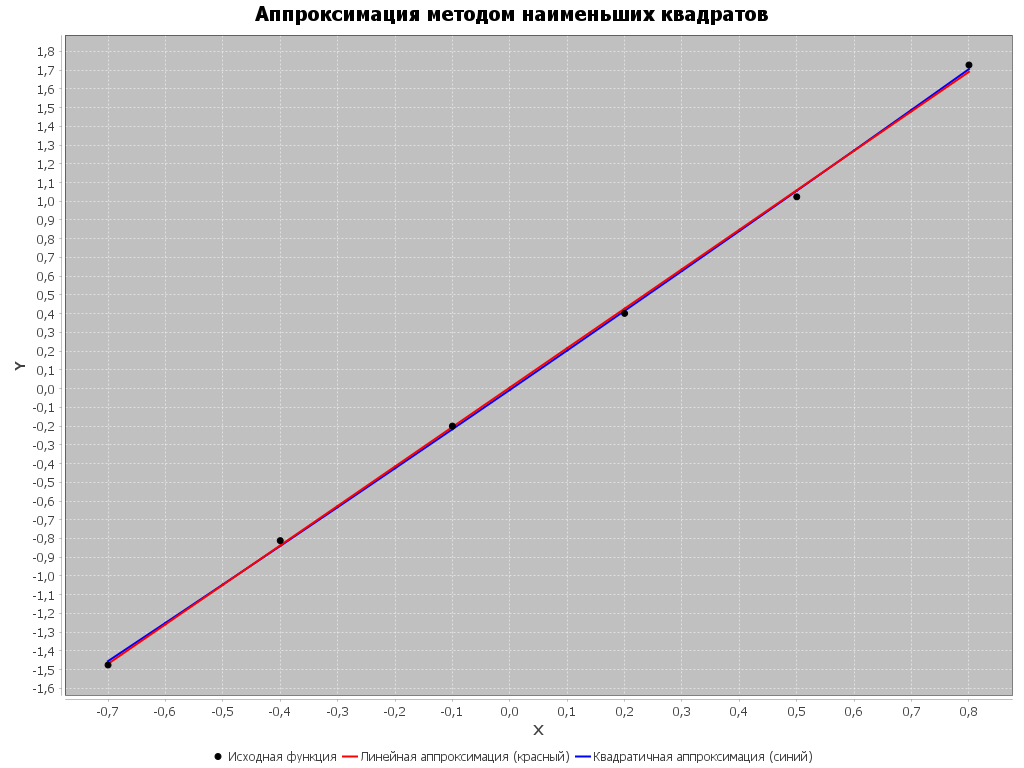
\includegraphics[scale=0.5]{chart}

\section*{Вывод}

\subsection*{Результаты аппроксимации}
\begin{itemize}
\item \textbf{Многочлен 1-ой степени}:
\[ y = 0.005526 + 2.106704x \]
Сумма квадратов ошибок: $\Phi_1 = 0.003942$

\item \textbf{Многочлен 2-ой степени}:
\[ y = -0.006992 + 2.101889x + 0.048147x^2 \]
Сумма квадратов ошибок: $\Phi_2 = 0.003241$
\end{itemize}

\subsection*{Анализ результатов}
\begin{enumerate}
\item \textbf{Сравнение точности}:
\begin{itemize}
\item Квадратичная модель показывает меньшую сумму квадратов ошибок ($\Delta\Phi = 0.000701$)
\end{itemize}

\item \textbf{Интерпретация коэффициентов}:
\begin{align*}
\text{Линейная модель:} &\quad \hat{y} \approx 2.1067x \\
\text{Квадратичная модель:} &\quad \hat{y} \approx 2.1019x + 0.0481x^2
\end{align*}
Квадратичный член вносит небольшой, но значимый вклад

\subsection*{Заключение}
\begin{itemize}
\item Обе модели адекватно описывают данные
\item Квадратичная аппроксимация демонстрирует ожидаемое улучшение точности
\item Выбор модели должен основываться на требованиях к точности и физическом смысле задачи
\end{itemize}
\end{enumerate}

\pagebreak
